%*******10********20********30********40********50********60********70********80

% For all chapters, use the newdefined chap{} instead of chapter{}
% This will make the text at the top-left of the page be the same as the chapter

\chap{Results: The Tuberculosis Co-authorship Network}
\label{chap:tb}
%\section{Background}
%Tuberculosis (TB) is a highly contagious and airborne infectious disease that is caused by \textit{Mycobacterium tuberculosis}. In 2015, TB was one of the top 10 causes of mortality worldwide. The global burden of TB worldwide is estimated at more than 1.8 million deaths including 0.4 million deaths among people living with HIV/AIDS in 2015. The disease has reportedly caused more deaths that same year than malaria and HIV/AIDS combined \cite{world_health_organization_global_2016}. \\
%At the Millenium Challenge summit of 2000, the Millenium Development Goal 6 (MDG6) was declared and aimed at a drastic reduction of the transmission of HIV/AIDS, Malaria and other diseases such as TB \cite{world_health_organization_mdg_2013}. According to the World Health Organization, the "World is on track" to achieving the MDG6 despite complicating factors such as the coinfection TB/HIV and the multidrug resistance in \textit{Mycobacterium Tuberculosis} \cite{world_health_organization_global_2016,falzon_world_2017,lynch_multidrug-resistant_2013}. 
%Despite those limitations, it is worth noting that the significant efforts made in terms of the increase in the global funding disturbement for TB \cite{global_fund_making_2011} has contributed to significantly scaling research efforts at reducing TB related mortality and morbidity. In the Republic of Benin where TB is the third major public health concern behind Malaria and HIV/AIDS, the increase in TB funding has led to a decrease of 0.8\% and 1.2\% respectively of the incidence and the annual death rate of TB in 2010 \cite{world_health_organization_global_2010}.\\ %For example, the year 2010 recorded the highest peak in the Global Fund disbursement for TB with an estimated 416 millions US dollars in 2010 \cite{global_fund_making_2011}.
%Achieving the MDG6 has resulted in change in public health policies accompanied by an increase in scientific research on Malaria, HIV/AIDS and TB \cite{world_health_organization_global_2010}. Scientific collaborations give researchers the opportunity to work and learn from each other. Such collaborations are further needed to overcome the overgrowing challenge of co-infections between HIV/AIDS and Tuberculosis \cite{corbett_growing_2003,gandhi_hiv_2010}. Identifying the main authors driving the publication efforts on TB and their collaborative patterns is an important basis for future public health strategies and to cooperative and translational scientific research initiatives \cite{gonzalez-alcaide_scientific_2012}. One approach to such an endeavour is the Social Network Analysis (SNA) of collaboration networks through co-authorship networks \cite{scott_social_2017,uddin_trend_2012}. \\
%The paradigm of co-authorship network is rooted in network theory, with the set of nodes represented by the authors and the set of edges describing the relationship between them \cite{newman_structure_2001}. The analyses of how complex TB co-authorship networks form and evolve in time is crucial for identifying leading researchers in the field, and describe their extant to collaborate with their peers as well as the impact of their research \cite{gonzalez-alcaide_coauthorship_2008}. An example of such investigation is illustrated in Newman scientific collaboration paper series on Biomedical research, physics and computer science co-authorship network \cite{newman_structure_2001,newman_scientific_2001-1,newman_scientific_2001,newman_coauthorship_2004}.\\
%The objective of this study was to analyze the authorship of scientific manuscripts on Tuberculosis in the Republic of Benin published in scientific journals indexed in the Web Of Science (WOS) from January 1, 1996 to December 31, 2016. By describing the structure of the TB network in Benin, we aim at providing a basis for research prioritization \cite{ghafouri_social_2014}, identification of prolific researchers, better design, strategic planning and effective implementation of research programs \cite{morel_co-authorship_2009}. 

\section{Data}
\label{sec:tb_data}
The literature search was conducted in the Web Of Science using combinations of TB related MeSH terms including "Tuberculosis", "Mycobacterium", "Infection". 
%We restricted the search to the period from 1996 to 2016 and to "Benin" for country. We further screened the papers in order to only select those published by Beninese authors, or papers published on TB from Benin. All published documents under considerations included at least one Author from Benin. No restriction was placed upon the document types. We first started querying with each term independently, we then combined the other terms so the query return the maximum number of results. The  Full citations information containing the authors' names, their institutional affiliations, the year of publication, as well as the number of times the document was cited were recorded as a bibliographic corpus in text format. After a second screening only research that have met the above listed inclusion criteria and that were published between January 1, 1996 and December 31, 2016 were selected. \\
The final query set (Table \ref{table: tb_search}) returned 109 records. The records were manually screened to verify the involvement of either an author from Benin or the use of data collected in Benin. Overall, 37 documents met the selection criteria. On average, there were 9.38 authors per published document. %\\

\begin{table}[h!]
\caption{TB Bibliographic Search Queries.}
\label{table: tb_search}
\centering \small
%\hspace{0.25}
\begin{tabular}{llc}
\toprule
Set & \multicolumn{1}{c}{Queries} & Results \\
\midrule
\#1 & TOPIC: (Tuberculosis) AND ADDRESS: (BENIN)  & 109 \\\\
\#2 & \begin{tabular}[c]{@{}l@{}}TOPIC: (Tuberculosis),\\Refined by: COUNTRIES/TERRITORIES: (BENIN )\end{tabular} & 77 \\\\
\#3 & \begin{tabular}[c]{@{}l@{}}TOPIC: (Mycobacterium Tuberculosis),\\AND ADDRESS: (Benin)\end{tabular} & 77 \\\\
\#4 & \begin{tabular}[c]{@{}l@{}}TOPIC: (Tuberculosis) OR TOPIC: (Infection) AND ADDRESS: (BENIN),\\Refined by: COUNTRIES/TERRITORIES: (BENIN)\end{tabular} & 89 \\
\midrule
Final Set & \#1 OR \#2 OR \#3 OR \#4 & 109\\
\bottomrule
\end{tabular}
\end{table}

After the Author Name Disambiguation, we identified 173 unique authors with a precision of 99.99\% and a recall of 99.99\%. The generated multigraph co-authorship network therefore contained 173 vertices (authors) and 1,937 parallel edges (collaborations). As displayed in figure \ref{tb_pubDist}, we can see the significant increase in publications, scientific collaborations and the number of authors involved in TB research from 2008 until 2016. This general upward trend seems to be linear from the year 2008 to 2016. \\

\begin{figure}[h!]
\centering
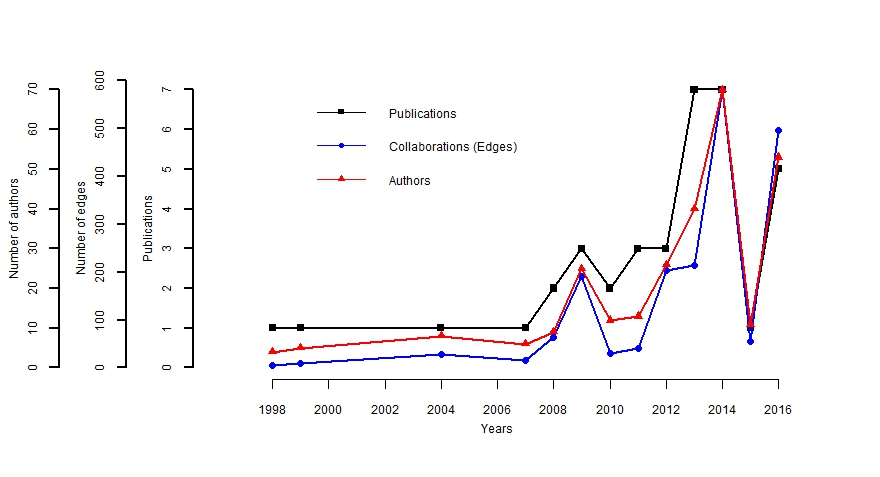
\includegraphics[scale=0.6]{Chapters/tb/pubDist}
\caption{Evolution of the published TB related documents, authors and collaborations from January 1996 to December 2016}
\label{tb_pubDist}
\end{figure}

\section{Descriptive Data Analysis}
\label{sec:tb_descstat}
For the multigraph network, the degree distribution ranged between 2 and 165 with an average degree distribution of 17.36 and a median of 15. In addition, there was a substantial number of vertices with low degrees (Fig. \ref{tb_fig1}). The log scale distribution of the degrees on figure \ref{tb_fig2} reveals that there was a tendency of prolific authors to collaborate with less prolific authors. 

\begin{figure}[h!]
\centering
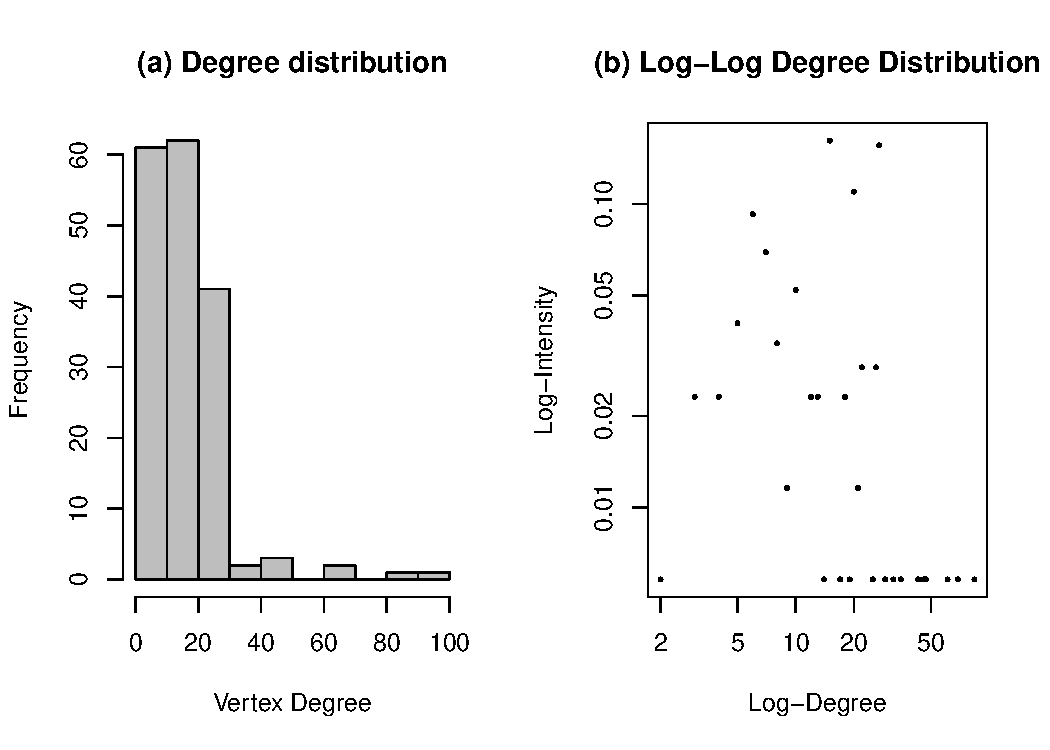
\includegraphics[scale=0.65]{Chapters/tb/degreeDistribution}
\caption{Degree distribution of the TB co-authorship network}
\label{tb_fig1}
\end{figure}

\begin{figure}[h!]
\centering
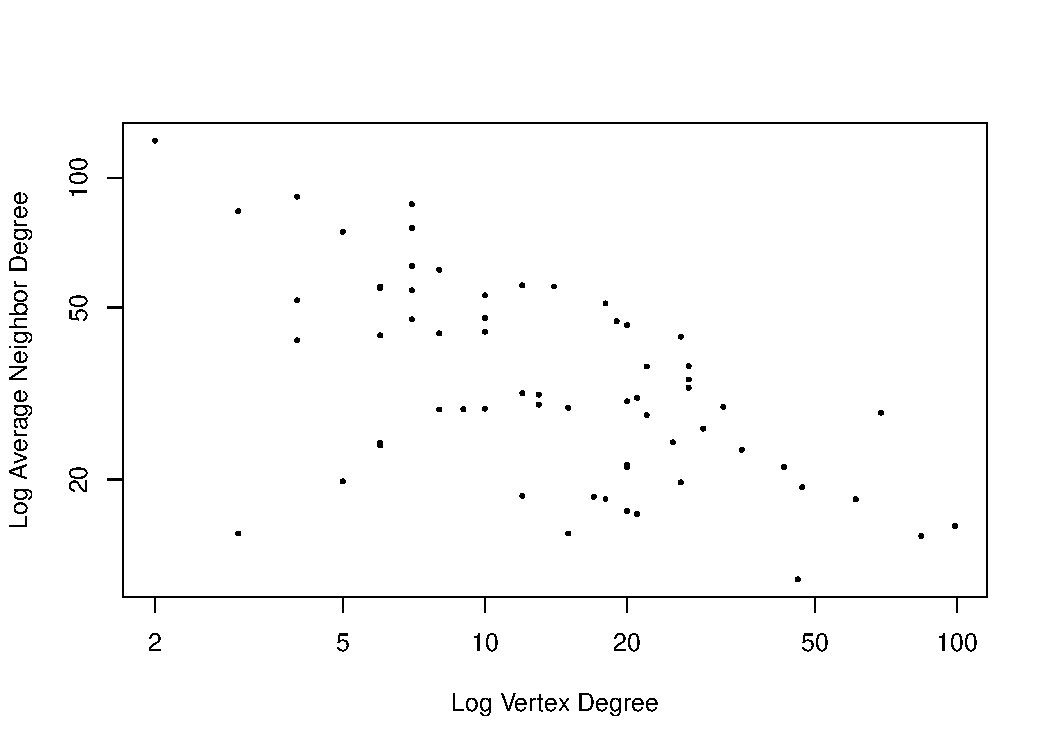
\includegraphics[scale=0.65]{Chapters/tb/logAvgDegree}
\caption{Log-Average Neighbor degree Distribution of the TB co-authorship network}
\label{tb_fig2}
\end{figure}

After converting the multigraph network in a weighted graph, the network results in a simple graph of 173 vertices and 1,502 weighted edges. Closeness centrality measures range between $3.68\times 10^{-5}$ and $3.28\times 10^{-4}$ with a median of $3.18\times 10^{-4}$. Betweenness measures range between 0 and 3,077 with a median of 12.49. A network visualization with the vertices' size proportional to betweenness centrality measures clearly reveals the presence of broker authors (Figure \ref{tb_fig5} and Table \ref{table: tb_list}). The median Eigenvectors is 0.087 and a mean of 0.138. Eigenvectors measures reveal the presence of author hubs in the network suggesting the presence of closed collaboration groups. Table \ref{table: tb_list} presents a list of the top 10 author hubs with the highest Eigenvectors values.\\
Edge betweenness centrality measures identify co-authorship collaboration ties that are important for the flow of information. Table \ref{table: tb_list} presents the top 10 most important collaboration ties for the flow of information in the TB co-authorship network in Benin. %\\

\begin{table}[h!]
\caption{List of the most important authors and collaborations in the Tuberculosis co-authorship network}
\label{table: tb_list}
\centering \small
\begin{tabular}{l}
  \toprule
\textbf{Top 10 Brokers}\\
%\hline
\hspace{20pt}AFFOLABI DISSOU\\
\hspace{20pt}GNINAFON MARTIN\\
\hspace{20pt}DE JONG BOUKE C\\
\hspace{20pt}TREBUCQ ARNAUD\\
\hspace{20pt}ODOUN MATHIEU\\
\hspace{20pt}ANAGONOU SEVERIN\\
\hspace{20pt}WACHINOU PRUDENCE\\
\hspace{20pt}FAIHUN FRANK\\
\hspace{20pt}KASSA FERDINAND\\
\hspace{20pt}ADE SERGE\\
\hline
\textbf{Top 10 most connected authors (Top 10 network hubs)}\\
\hspace{20pt}GNINAFON MARTIN\\
\hspace{20pt}AFFOLABI DISSOU\\
\hspace{20pt}ANAGONOU SEVERIN\\
\hspace{20pt}MERLE CORINNE S C\\
\hspace{20pt}TREBUCQ ARNAUD\\
\hspace{20pt}OLLIARO PIERO L\\
\hspace{20pt}RUSTOMJEE ROXANA\\
\hspace{20pt}LO MAME BOCAR\\
\hspace{20pt}LIENHARDT CHRISTIAN\\
\hspace{20pt}HORTON JOHN\\
\hline
\textbf{Top 10 most important edges for information flow}\\
\hspace{20pt}ODOUN MATHIEU -- GNINAFON MARTIN\\
\hspace{20pt}FAIHUN FRANK -- DE JONG BOUKE C\\
\hspace{20pt}ODOUN MATHIEU -- TREBUCQ ARNAUD\\
\hspace{20pt}ZELLWEGER J P -- GNINAFON MARTIN\\
\hspace{20pt}TREBUCQ ARNAUD -- ADJONOU CHRISTINE\\
\hspace{20pt}ODOUN MATHIEU -- WACHINOU PRUDENCE\\
\hspace{20pt}AFFOLABI DISSOU -- BAHSOW OUMOU\\
\hspace{20pt}AFFOLABI DISSOU -- TOUNDOH N\\
\hspace{20pt}AFFOLABI DISSOU -- BEKOU W\\      
\hspace{20pt}AFFOLABI DISSOU -- MAKPENON A\\
\hline
\textbf{Weak articulation point}\\
\hspace{20pt}WACHINOU PRUDENCE\\
\bottomrule
\end{tabular}
\end{table}

\subsection{Network Cohesion}
Overall, 28 maximal cliques were detected in the network among which 1 clique of size 10, 2 cliques of size 5, and 2 cliques of size 4. The largest clique has size 10. \\
The TB co-authorship network has a density of 0.10095 indicating that the baseline probability of collaboration tie formation is 10.095\%. The network also has a transitivity of 0.6305 meaning that 63.05\% of the connected triples in the network are close to form triangles. The transitivity measures the global clustering of the network.\\
The network is not connected and a census of all the connected components within the network reveals the existence of a giant component that dominates all the other connected components. The giant component of the TB co-authorship network includes 90.8\% (157 vertices) of all the vertices in the network with the other components alone carrying less than 0.1\% of the vertices in the network (Fig. \ref{tb_fig5}). 

\begin{figure}[h!]
\centering
\hspace{1.5cm}
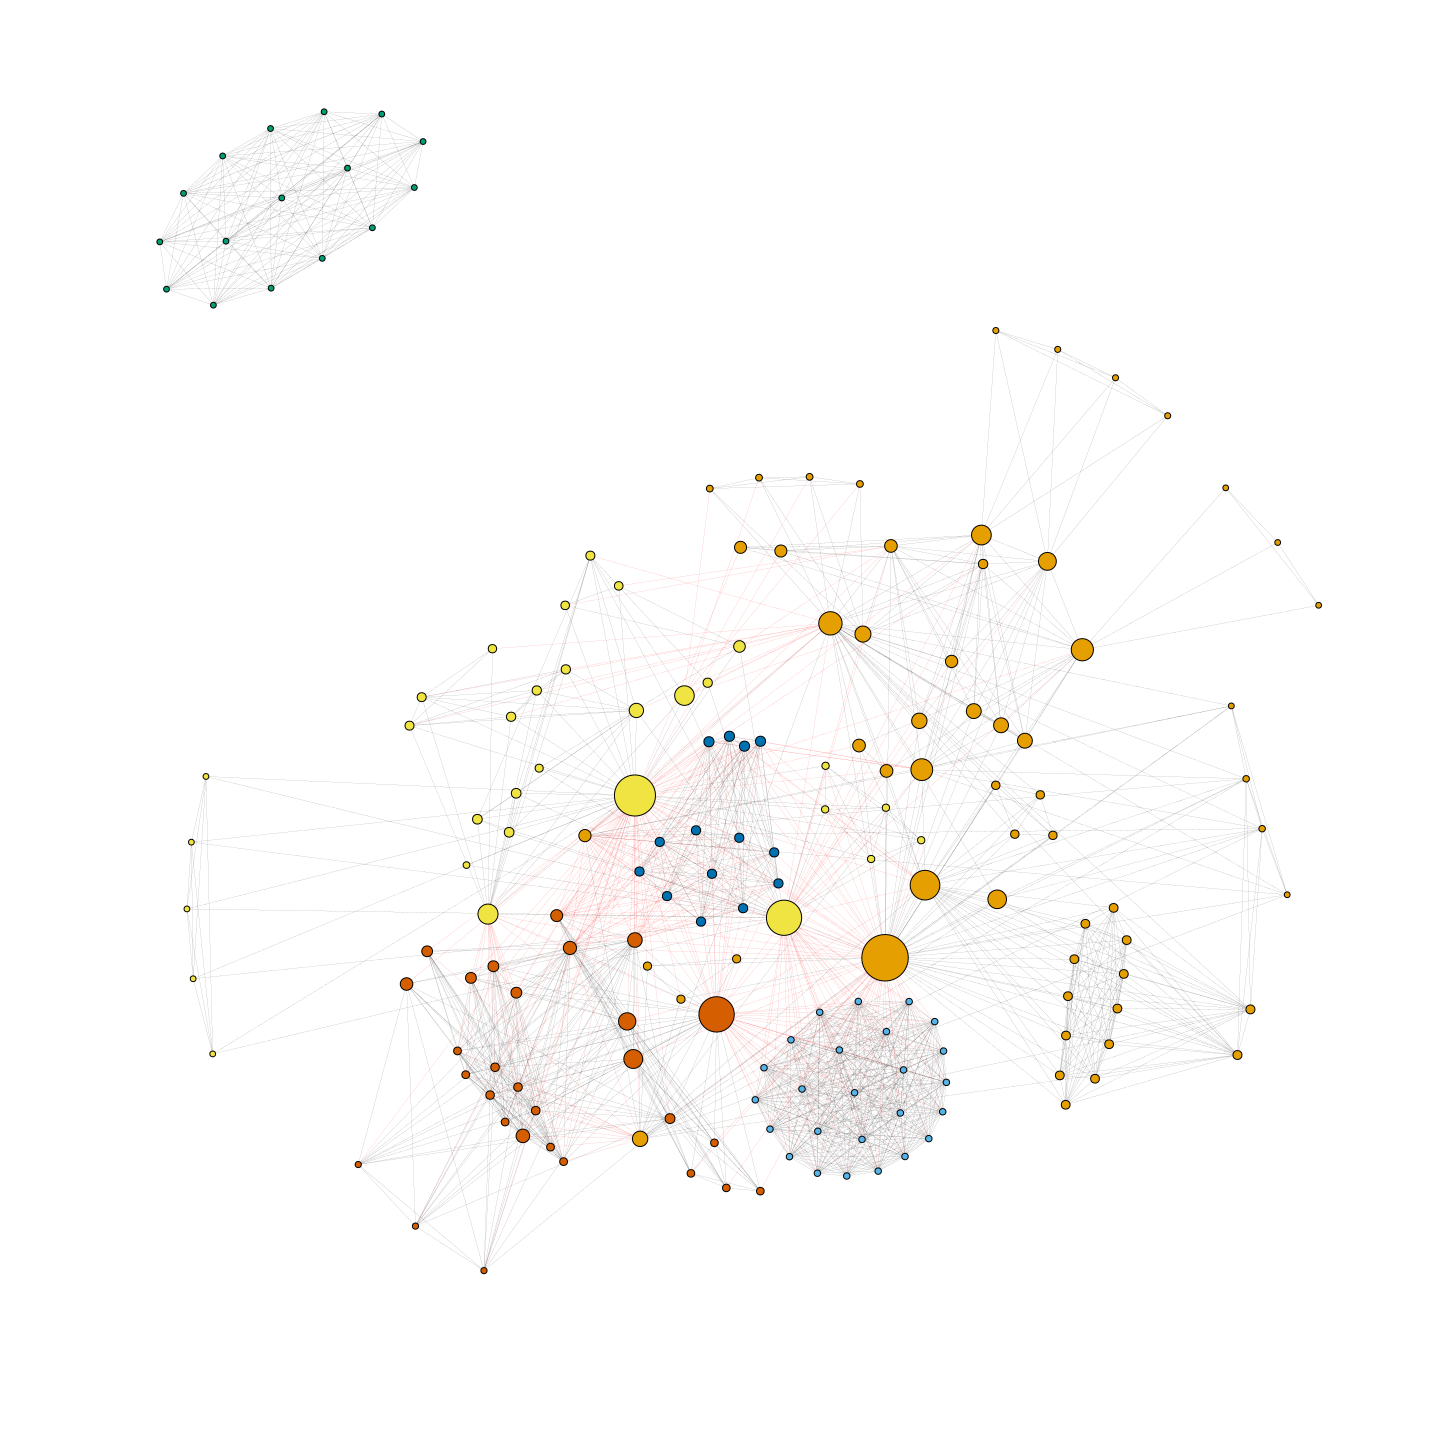
\includegraphics[scale=0.35]{Chapters/tb/tbnet}
\caption{Topological Structure of the Tuberculosis co-authorship network. Authors (vertices) of the same color belong to the same research community or cluster}
\label{tb_fig5}
\end{figure}

Information flow assessment of the network via cut vertices reveals the existence of a single author as the most vulnerable vertex in the network (Table \ref{table: tb_list}). The cut vertex constitute the weak articulation point of the TB co-authorship network. Cut vertices represent a measure of the vulnerability of the network \cite{kolaczyk_statistical_2014}.\\
The agglomerative hierarchical clustering method identifies 6 different clusters in the network. Sizes of the clusters range between 14 and 58 authors. Out of the 6 research clusters detected, 5 are in the giant component. Figure \ref{tb_fig5} displays the giant component of the network with each different colors representing each of the 6 clusters. %\\

%\pagebreak
\section{Modeling}
\subsection{Mathematical Modeling}
From the hierarchical clustering method of community detection, 6 different clusters were detected in the co-authorship network out of which 5 form a giant component. We performed 1,000 Monte Carlo based simulations to test the significance of this observed characteristic of the TB co-authorship network. Figure \ref{tb_fig3} clearly demonstrates that the number of communities detected is unusual from the perspective of both Classical random graphs and generalized random graphs (p-value < 0.0001). From the Classical random graph model, the expected number of communities was 4.734 (95\%CI: 4.70 -- 4.77). Similarly, the expected number of communities from the generalized random graph model is 5.34 (95\%CI: 5.29 -- 5.38).

\begin{figure}[h!]
\centering
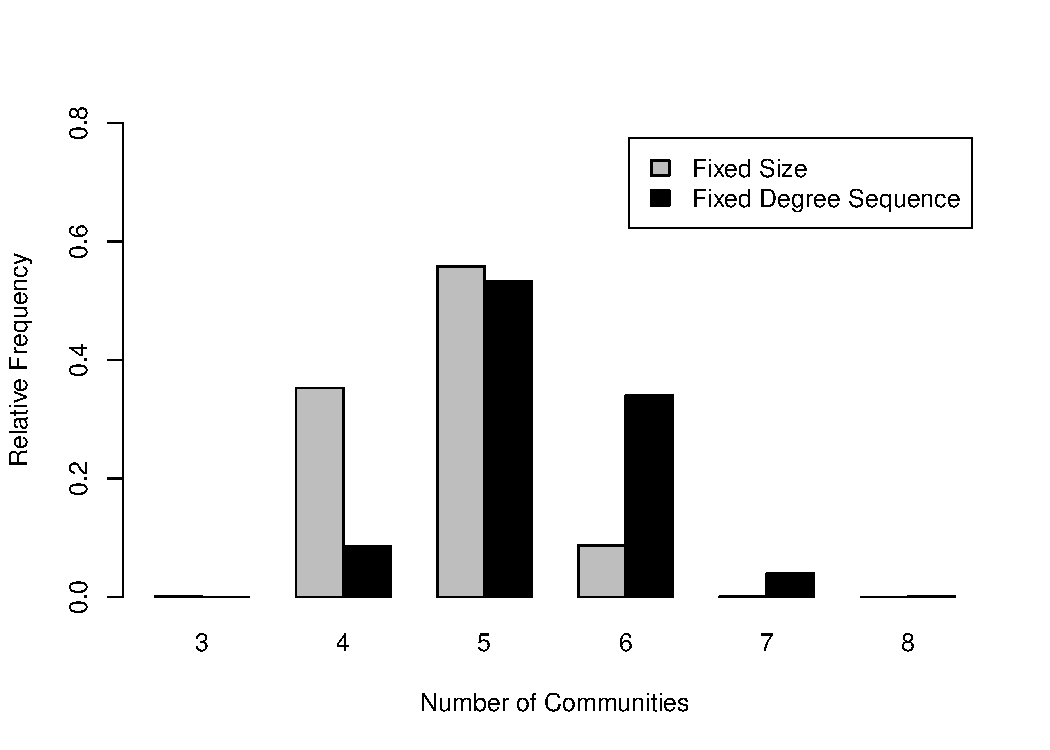
\includegraphics[scale=0.65]{Chapters/tb/randomComm}
\caption{Monte-Carlo simulations of the TB network: Number of detected communities by the random graph models}
\label{tb_fig3}
\end{figure}

Figure \ref{tb_fig4} displays the number of detected clusters or research communities using the Barab\'asi-Albert's preferential attachment and the Watts-Strogatz models. Here too, the observed number of communities was extreme per both models (p-value < 0.0001). The expected number from the Watts-Strogatz model simulations is 3.017 (95\%CI: 3.01 -- 3.03) and 13.77 (95\%CI: 13.70 -- 13.85) from the Barab\'asi-Albert model simulations. 

\begin{figure}[h!]
\centering
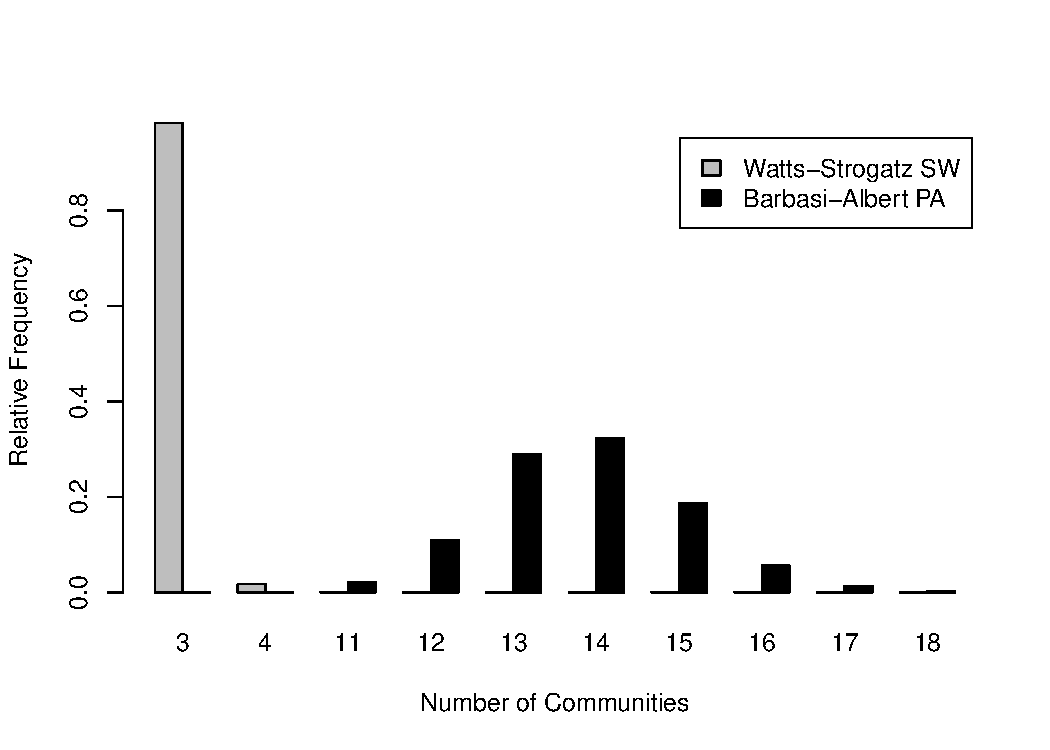
\includegraphics[scale=0.65]{Chapters/tb/mechanisticComm}
\caption{Monte-Carlo simulations of the TB network: Number of detected communities by the Watts-Strogatz and the Barab\'asi-Albert models}
\label{tb_fig4}
\end{figure}

We also compared the clustering coefficient and the average shortest-path length. Let's recall that the observed clustering coefficient is 0.614. On one hand, there was substantially more clustering in our TB co-authorship network than expected from both random graph models (p-value < 0.0001). The expected clustering coefficients was 0.10087 (95\%CI: 0.10068 -- 0.10107) and 0.1937 (95\%CI: 0.1934 -- 0.1939) respectively for the classic random graph and the generalized random graph models.\\
On the other hand, there was substantially less clustering in our TB co-authorship network than expected from the Watts-Strogatz Small World model which expected clustering was 0.7259 (95\%CI: 0.7258 -- 0.7260).\\
We observed an average shortest-path length of 2.126 in the TB co-authorship network. This observed shortest-path length is significantly larger than what was expected from the random graph models (p-value < 0.0001) and significantly lower than what was expected from Watts-Strogatz small world model and the Barab\'asi-Albert preferential attachment model (p-value < 0.0001).\\
The average shortest-path length was 2.0548 (95\%CI: 2.0546 -- 2.0550) and 2.072 (95\%CI: 2.0715 -- 2.0726) respectively for the classic random graph and the generalized random graph models.\\For the Watts-Strogatz small world and the Barab\'asi-Albert models, the average shortest-path length is respectively 2.623 (95\%CI: 2.616 -- 2.631) and 6.06 (95\%CI: 6.03 -- 6.09).\\~\\
We performed the same simulations on the giant component of the network with similar results leading to the same outcomes.

\subsection{Statistical Modeling}
%For the purposes of modeling the temporal dynamic of collaboration ties formation, we subset the network in different temporal snapshots. We subset the network, generating snapshots in a certain way that balanced the number of edges across the years. Such an uneven subsetting improved the robustness of our models and ensured model convergence. We ended up with 7 snapshots representing respectively the following timestamps: 1996 -- 2006, 2007 -- 2009, 2010 -- 2011, 2012 -- 2013, 2014, 2015 and 2016. %\\
%Figure \ref{fig:tb_dynNetwork} displays the topological structure of the snapshots of the different time steps.

\subsubsection{Stochastic Block Model}
\label{sec:tb_results_sbm}
The SBM identifies 14 classes with a degree of latitude of 9 to 14 classes being reasonable (See ICL plot on figure \ref{fig:tb_sbmgof}).

\begin{figure}[h!]
\centering
\hspace*{-1cm}
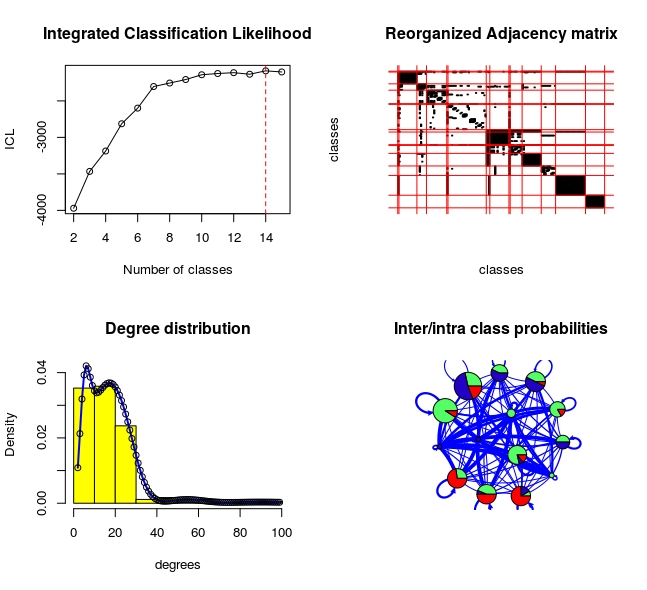
\includegraphics[scale=0.85]{Chapters/tb/statMod/tb_sbm}
\caption{Summary of the goodness-of-fit of the SBM analysis on the Tuberculosis co-authorship network.}
\label{fig:tb_sbmgof}
\end{figure}

The fitted SBM describes well the observed degree distribution. The vertices in the network depicting the inter/extra probabilities represent the 14 identified classes, with each one of them divided into a pie chart displaying the proportion of authors of international affiliations (lightgreen), authors of regional or other African affiliations (red), and authors affiliated to Beninese research institutions (blue). Generally, the dominance across the classes of international and regional players is observed. From the inter/intra probability network shows denser inter class ties. Looking at the pie charts, we can see that the classes are heterogeneous with most of the classes having the same sizes (\ref{fig:tb_sbmgof}). Figure \ref{fig:tb_sbmdist} presents the distribution of the classes by affiliation types. \\

\begin{figure}[h!]
\centering
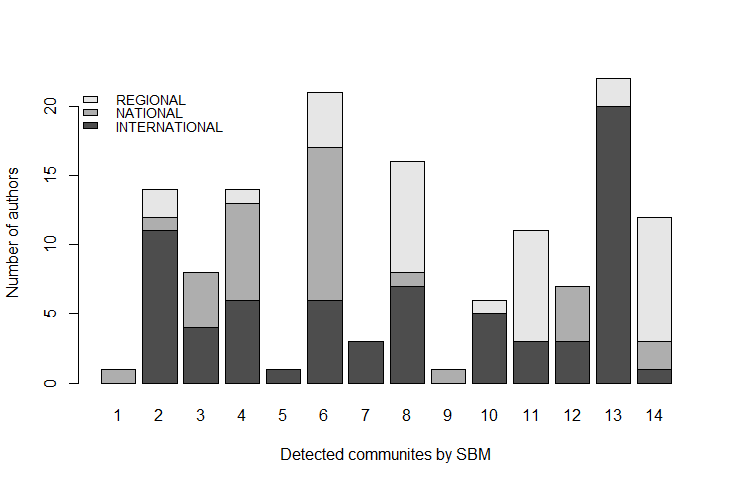
\includegraphics[scale=0.8]{Chapters/tb/statMod/tb_barplot2}
\caption{Distribution of national, international and regional authors by communities detected by the SBM in the TB network.}
\label{fig:tb_sbmdist}
\end{figure}

%On figure \ref{fig:hiv_sbmgof2}, we present the SBM results emphasizing the largest classes (with more than 20 members). Here, we can confirm that smaller classes tend to collaborate more among themselves and in-class collaborations tend to occur more.
%
%\begin{figure}[h!]
%\centering
%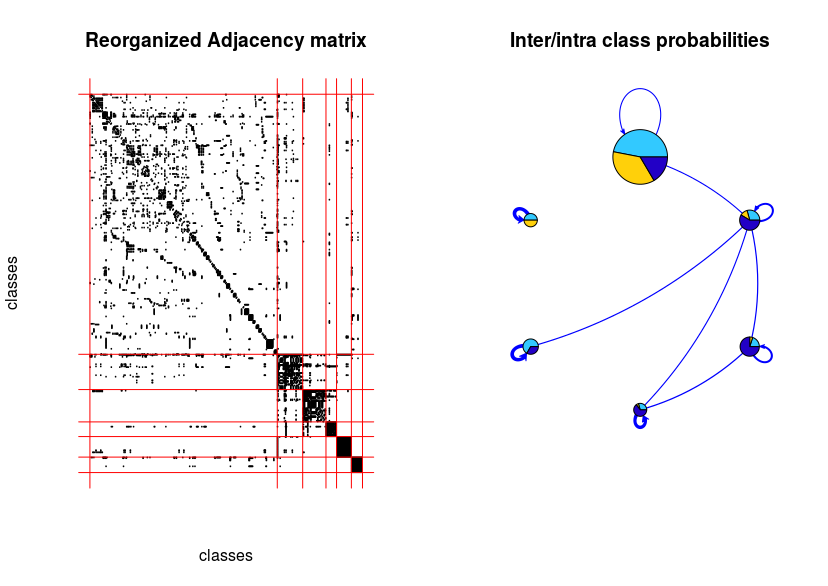
\includegraphics[scale=0.65]{Chapters/hiv/statMod/hiv_sbm2}
%\caption{Summary of the goodness-of-fit of the SBM analysis highlighting interactions between the largest classes of the HIV/AIDS co-authorship network.}
%\label{fig:hiv_sbmgof2}
%\end{figure}

\subsubsection{Exponential Random Graph Model}
\label{sec:tb_results_ergm}
We fit multiple ERGMs (Table \ref{tab:tb_ergm}). In the null model (model 1), the inverse logit of the coefficient associated with the intercept (edge term) is $0.10$ which is the baseline probability of collaboration tie establishment and also the density of the TB co-authorship network.

\begin{table}
\begin{center}
\hspace*{-1cm}
\small
\begin{tabular}{@{}lcclclcl@{}}
\toprule
           &  & Model 1 &  & Model 2  &  & Model 3\\ \cmidrule{3-3} \cmidrule{5-5} \cmidrule{7-7}            &  & Estimate ($SE$) &  & Estimate ($SE$)  &  & Estimate ($SE$) \\ \midrule
           Network structural predictor &  &   &  &  &  \\
\hspace{10pt}Intercept(edge) & & $-2.19 \; (0.03)^{***}$ & & $-7.84 \; (0.16)^{***}$ & & $-7.86 \; (0.17)^{***}$ \\ \\
Number of times cited        & &       --  & & $\hspace{6pt}0.01 \; (0.00)^{***}$ &  & $\hspace{6pt}0.01 \; (0.00)^{***}$  \\
Number of collaborations     & &  --  & & $\hspace{6pt}0.08 \; (0.00)^{***}$ &  & $\hspace{6pt}0.07 \; (0.00)^{***}$  \\
Number of publications       & &  --  & & $-0.05 \; (0.01)^{**~~}$ &  & $\hspace{6pt}0.01 \; (0.02)^{~~~~}$   \\
Homophily on cluster assignment &  &   --  &  & $\hspace{6pt}6.02 \; (0.13)^{***}$ &  & $\hspace{6pt}6.12 \; (0.14)^{***}$  \\
Homophily on collaboration type   &   & -- &   & $\hspace{6pt}0.83 \; (0.10)^{***}$ &  & $\hspace{6pt}0.90 \; (0.10)^{***}$  \\ \\
Factor attribute effect (collaboration type) &  &    &  &  &   &   \\
\hspace{10pt}International   &  & --   &  & --   &  & $REF$\\
\hspace{10pt}National        & &  --   &  &  -- & & $-0.40 \; (0.09)^{***}$ \\
\hspace{10pt}Regional        & &  --   &  & --  & & $\hspace{6pt}0.22 \; (0.08)^{**}$   \\
\midrule
AIC           &  & $\hspace{6pt}9737.42$  &  & $\hspace{6pt}3776.48$  &  & $\hspace{6pt}3747.34$ \\
BIC           &  & $\hspace{6pt}9745.03$  &  & $\hspace{6pt}3822.12$  &  & $\hspace{6pt}3808.20$ \\
Log Likelihood   &  & $-4867.71$        &  & $-1882.24$         &    & $-1865.67$ \\
\bottomrule
\multicolumn{4}{l}{\scriptsize{$^{***}p<0.001$, $^{**}p<0.01$, $^*p<0.05$}}
\end{tabular}
\caption{ERGM of the TB co-authorship network.}
\label{tab:tb_ergm}
\end{center}
\end{table}

Model 2 including all nodal variables, a homophily term on collaboration type and on cluster assignment improved tremendously compared to model 1 (See AIC, BIC and model likelihood in table \ref{tab:tb_ergm}). We note a decrease in the edge effect (Coefficient $=-7.84$, $p<0.001$) with the associated conditional probability (given all the other terms in the model) estimated at $0.039\%$. For the remaining terms in model 2, we observed a positive and significant effect except for the number of publications. Model 3 including the collaboration type as factor term, improved substantially compared to model 2. We therefore chose model 3 as our final model. One unit increases the number of citation, increases the odds of collaboration ties establishment by $1\%$. A one unit increase in the number of collaborations is associated with a $7.25\%$ increase in the odds of collaboration ties establishment. The coefficient associated with the number of publications is insignificant. Model 3 further proves that the process underlying the structure of the TB co-authorship network in Benin is mainly driven by homophily on cluster assignment or membership to a research community or group (Coefficient $=6.12$, $p<0.001$). The conditional probability of any two authors belonging to the same research group is estimated at $14.93\%$ compared to the baseline probability of $10\%$. The same probability changes to $30.15\%$ after adjustment by the collaboration type, and $32.08\%$ after adjusting for the number of citations, collaborations and publications. Compared to research affiliated to international institutions, researchers affiliated to Beninese institutions have $49.2\%$ average decrease in the odds of collaboration tie establishment. This average decrease is not statistically significant ($p>0.05$). For researchers affiliated to institutions other than Beninese institutions, the odds of collaboration tie establishment increase on average by $24.05\%$ compared to internationally affiliated researchers. Overall, model 3 estimated the probability of collaboration ties formation at $32.08\%$ for international researchers, $24.05\%$ for national researchers and $37.05\%$ for regional players. \\
Unfortunately, none of the models containing endogenous ERGM terms and/or the dyadic variables, attained convergence, we do not present those results in table \ref{tab:tb_ergm}.

\begin{sidewaysfigure}
%\begin{figure}[!h]
\centering
\hspace*{-1cm}
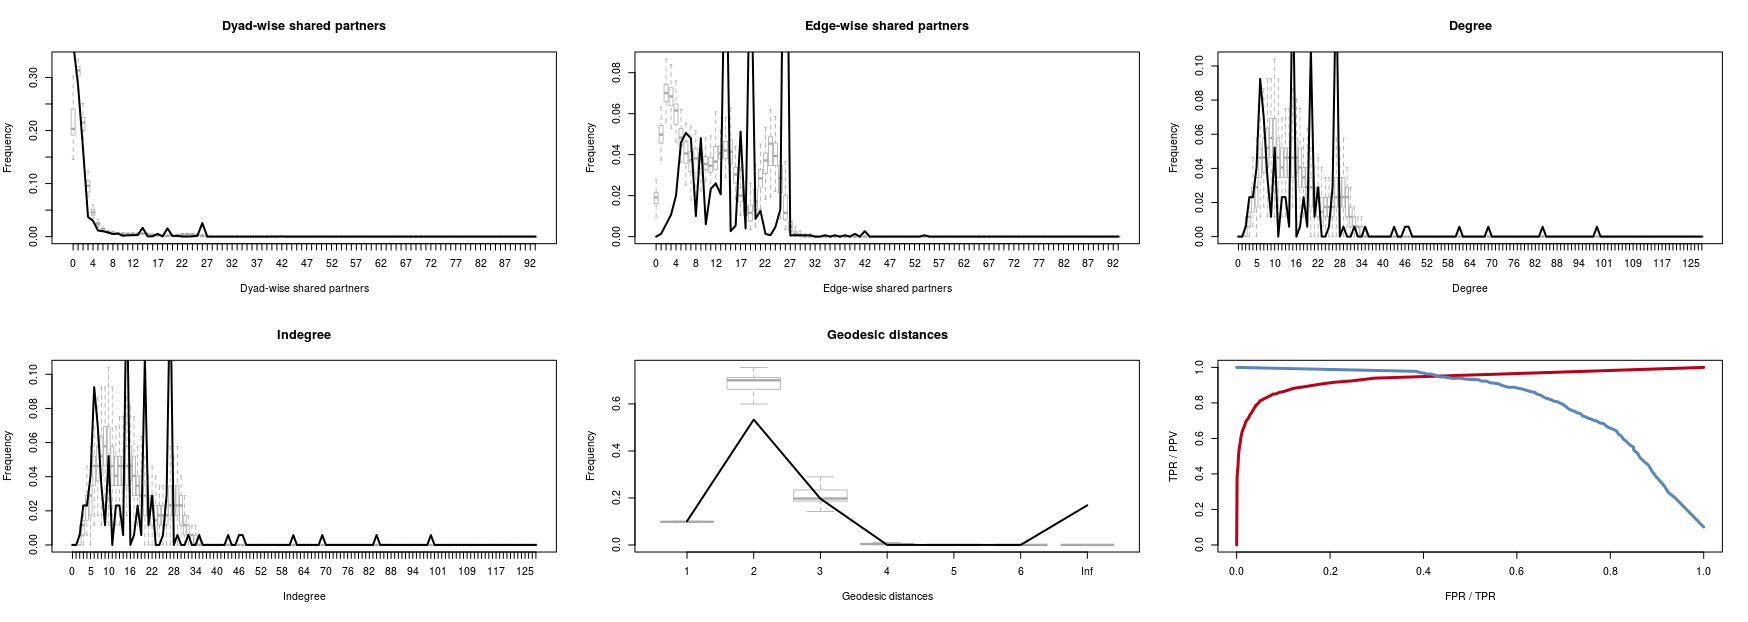
\includegraphics[height=14cm,width=22cm]{Chapters/tb/statMod/tb_ergm_gof2}
\caption{ERGM goodness-of-fit of final model 3 assessment on the TB co-authorship network.%\\
%The observed properties are depicted by the black lines. Gray lines with circles represent the 95\% confidence intervals for the simulated network properties. Goodness-of-fit is asserted when the black lines lie in-between the confidence intervals lines.
}
\label{fig:tb_ergm-gof}
%\end{figure}
\end{sidewaysfigure}

Figure \ref{fig:tb_ergm-gof} presents the goodness-of-fit of the final model 3. It appears that the ERGM fits somewhat poorly the observed TB co-authorship network in terms of edge-wise, dyad-wise shared partners, degree, geodesic distances, triad census. Meanwhile, it displays a $93.7\%$ for the ROC model (in red) and $80.9\%$ for the Precision Recall (PR) model.

\subsubsection{Temporal Exponential Random Graph Model}
\label{sec:tb_results_tergm}
We subset the cumulative observed network in five snapshots according to the following time spans: 1996 -- 2008, 2009 -- 2011, 2012 -- 2013, 2014 -- 2015 and 2016. In figure \ref{fig:tb_dynNetwork}, we show the topological structure of the network snapshots for the different time steps.

\begin{figure}[!ht]
\hspace{-1.25cm}
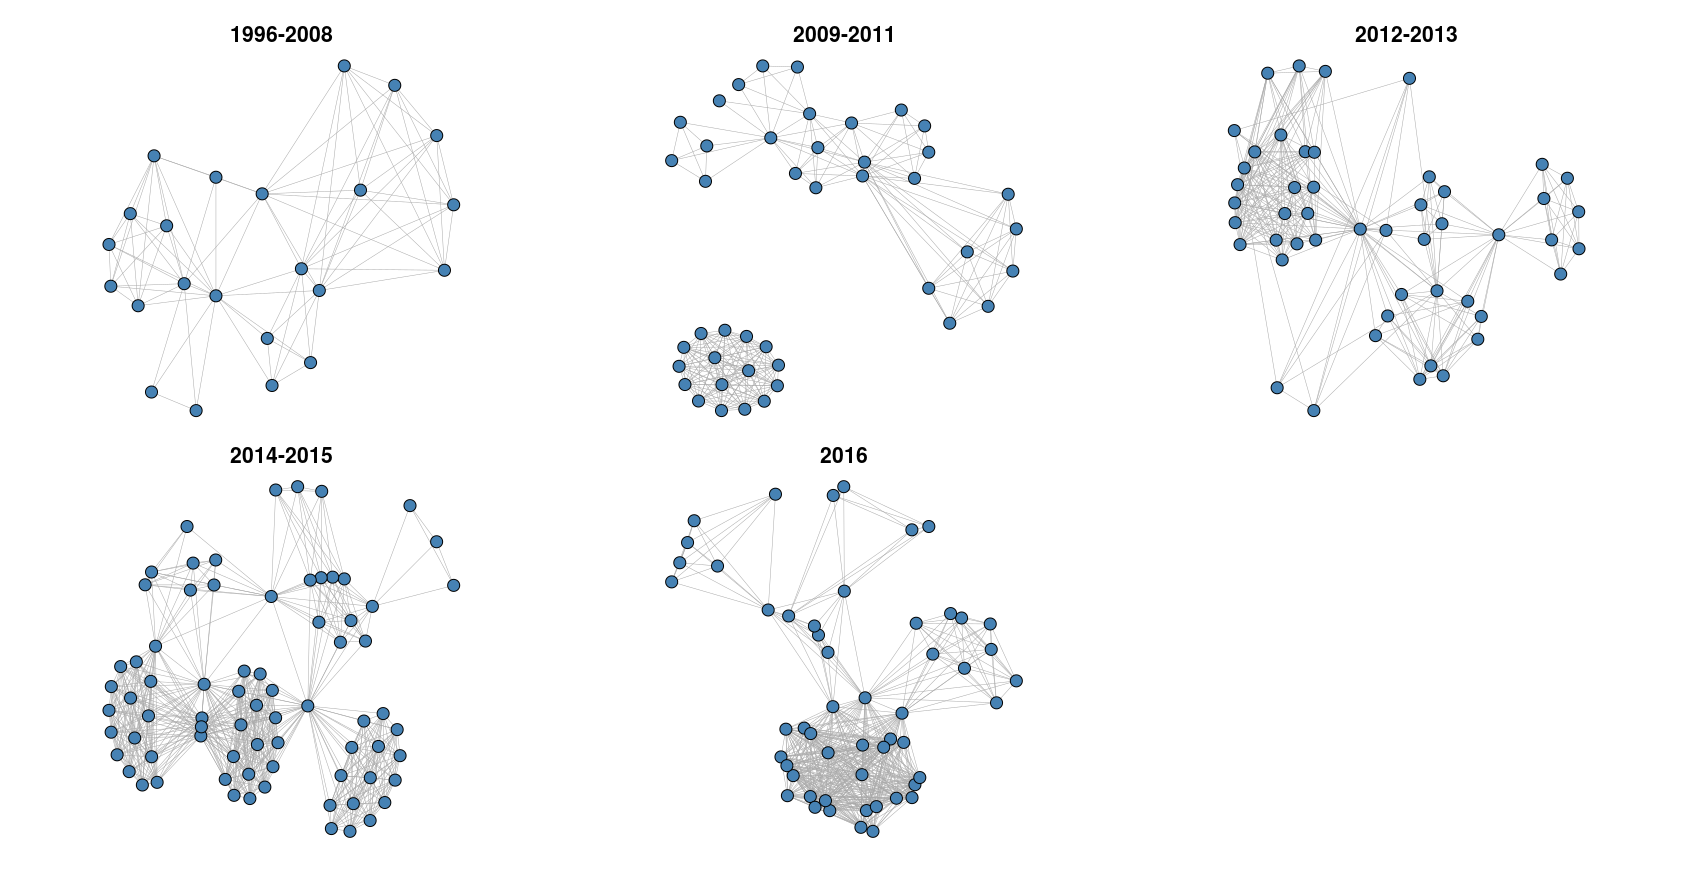
\includegraphics[scale=0.4]{Chapters/tb/statMod/tb_dynNetwork}
\caption{Topological structure of the different snapshots of the TB co-authorship network.}
\label{fig:tb_dynNetwork}
\end{figure}

Table \ref{tab:tb_tergm} summarizes the results of the different temporal models fit to the observed snapshots of the network. The coefficient for the edge term in the null pooled ERGM model 1 is estimated at $-3.75$ with an associated baseline pooled probability of collaboration tie formation of $2.30\%$, which is lower than the density of the observed cumulative TB network.\\
Model 2 adjusts for the nodal variables and the homophily terms improved slightly over the null model 1. Model 3 adjusted model 2 by including a factor attribute effect on the collaboration type with a slight improvement over model 2. Unlike the final model of the ERGM, we observed in model 3, a significant decrease of $23.4\%$ in the odds of researchers affiliated with Beninese institutions to collaborate compared to international researchers. This percentage decrease changes to $40.5\%$ after adjusting for the temporal dependencies in model 4. \\
We chose Model 4 as our final model because it significantly improved over model 3. The results of model 4 confirm our observation from the ERGM results that the process of collaboration tie establishment in the TB network is mainly driven by homophily on collaboration type and on membership to research groups or communities. \\
Temporal dependencies effects proved significant in the final model. A significantly positive dyadic stability effect accompanied with a significantly negative linear trends effect is observed. For dyadic stability, the coefficient is $0.44$ meaning that the odds of existent and non existent collaboration ties at one time point to remain the same at the next time point increased on average by $35.6\%$. In other words, the odds of new collaboration ties and non-ties to occur from one time point to another is $64.4\%$. Overall, the probability of international authors to establish a stable collaboration tie is $15.71\%$ versus $11.71\%$ and $16.11\%$ respectively for national and regional researchers.\\
The goodness-of-fit assessment of the final TERGM model 4 is presented in figure \ref{fig:tb_tergm-gof}. Regarding the endogenous network statistics, we observe a better fit of the final TERGM model 4 compared to the final ERGM model 3. In other words, the simulated network by model 4 show a good fit to the observed TB network data. The AUC of the ROC curve of model 4 (see dark red curve on subfigure 6) is estimated at $83.2\%$ meaning that $83.2\%$ of the times, model 4 accurately predicts ties in the last snapshot. While this performance is lower than the performance of the final ERGM model 3 from the previous section, the walktrap and edge betweenness modularity distributions from model 4 predicted well the observed ones. Finally, the walktrap community comembership prediction displays an AUC of $71.4\%$ (see dark red curve on subfigure 5).

\begin{table}
\begin{center}
\caption{Temporal ERGM of the TB co-authorship network.}
\label{tab:tb_tergm}
\hspace*{-1cm}
\scriptsize
\begin{tabular}{@{}lcclclclcl@{}}
        \toprule
           &  & Model 1 &  & Model 2  &  & Model 3 &  & Model 4\\ \cmidrule{3-3} \cmidrule{5-5} \cmidrule{7-7} \cmidrule{9-9}
           &  & Estimate ($SE$) &  & Estimate ($SE$)  &  & Estimate ($SE$) &  & Estimate ($SE$)\\
\midrule
Network structural predictor & & & & & & & & \\
\hspace{10pt}Intercept(edge)    &  & $-3.75 \; (0.02)^{***}$ & & $-10.07 \; (0.15)^{***}$ & & $-10.01 \; (0.16)^{***}$ & & $-8.62 \; (0.28)^{***}$ \\\\
Number of times cited       &  &       --    &  & $\hspace{6pt}0.00 \; (0.00)^{*~~~}$   &  & $\hspace{6pt}0.00 \; (0.00)^{~~~~}$      &  & $-0.00 \; (0.00)^{**~}$  \\
Number of collaborations    &  &         --  &  & $\hspace{6pt}0.14 \; (0.00)^{***}$ &  & $\hspace{6pt}0.14 \; (0.00)^{***}$ &  & $\hspace{6pt}0.16 \; (0.00)^{***}$  \\
Number of publications      &  &      --     &  & $\hspace{6pt}0.68 \; (0.03)^{***}$ &  & $\hspace{6pt}0.72 \; (0.03)^{***}$ &  & $\hspace{6pt}0.57 \; (0.03)^{***}$  \\
Homophily on cluster assignment   &  & --     &  & $\hspace{6pt}5.24 \; (0.11)^{***}$ &  & $\hspace{6pt}5.23 \; (0.11)^{***}$ &  & $\hspace{6pt}5.40 \; (0.13)^{***}$  \\
Homophily on collaboration type   &  &   --   &  & $\hspace{6pt}0.69 \; (0.08)^{***}$ &  & $\hspace{6pt}0.69 \; (0.08)^{***}$ &  & $\hspace{6pt}0.73 \; (0.09)^{***}$  \\\\
Factor attribute effect (collaboration type) & & & & & & & & \\
\hspace{10pt}International & & -- & & -- & & $REF$ & & $REF$ \\
\hspace{10pt}National  &  &  --   &  &   --   &  & $-0.21 \; (0.07)^{**~}$ &  & $-0.34 \; (0.08)^{***}$ \\
\hspace{10pt}Regional &  &    --  &  &   --   &  & $\hspace{6pt}0.03 \; (0.07)^{~~~~}$ &  & $\hspace{6pt}0.03 \; (0.08)^{~~~~}$    \\\\
Temporal dependencies & & & & & & & & \\
\hspace{10pt}Dyadic stability  &  &  --  &  &  -- &  &   --  &  & $\hspace{6pt}0.44 \; (0.07)^{***}$  \\
\hspace{10pt}Linear trends     &  &  --  &  &  -- &  &   --  &  & $-0.36 \; (0.06)^{***}$ \\
\midrule
AIC    & & $\hspace{6pt}431184.00$   & & $\hspace{6pt}419860.54$ & & $\hspace{6pt}419853.82$ & & $\hspace{6pt}253170.25$   \\
BIC    & & $\hspace{6pt}431205.66$ & & $\hspace{6pt}419936.36$ & & $\hspace{6pt}419951.30$ & & $\hspace{6pt}253284.48$    \\
Log Likelihood    & & $-215590.00$ & & $-209923.27$ & & $-209917.91$ & & $-126574.12$ \\
\bottomrule
\multicolumn{5}{l}{\scriptsize{$^{***}p<0.001$, $^{**}p<0.01$, $^*p<0.05$}}
\end{tabular}
\end{center}
\end{table}

\begin{sidewaysfigure}
%\begin{figure}[!h]
\centering
\hspace*{-1cm}
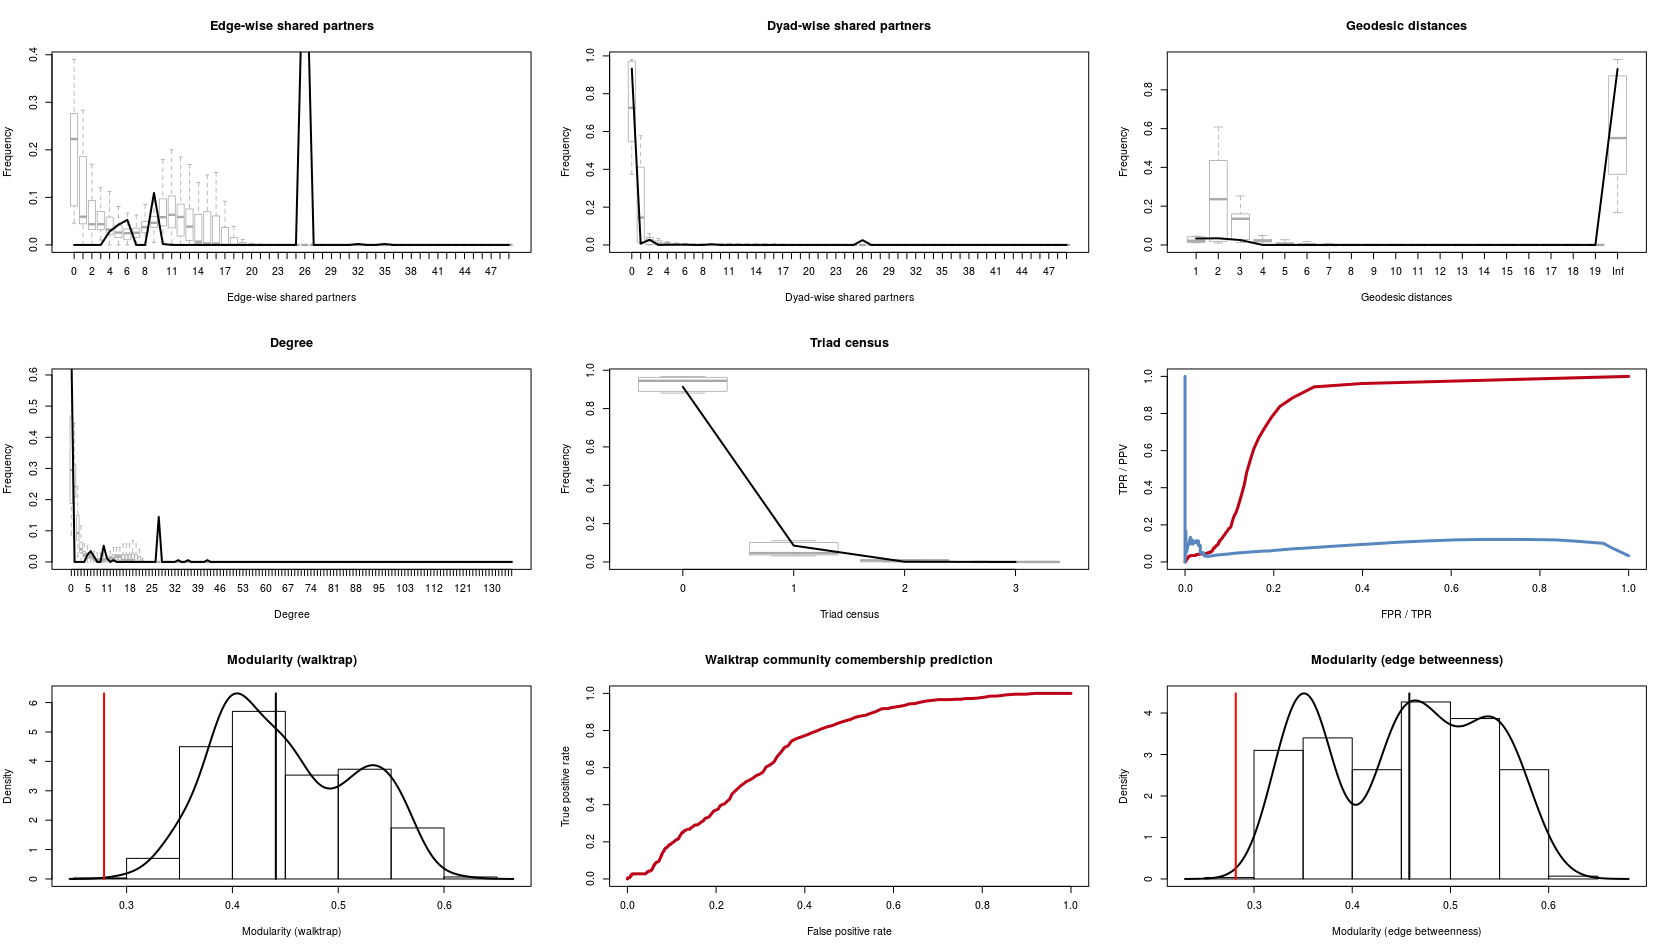
\includegraphics[scale=0.5]{Chapters/tb/statMod/tb_tergm_gof}
\caption{Goodness-of-fit assessment for the final TB TERGM Model 4 with temporal dependencies of the TB co-authorship network.}
\label{fig:tb_tergm-gof}
%\end{figure}
\end{sidewaysfigure}

%\pagebreak
\pagebreak
\subsubsection{Latent Network Model}
\label{tb_sec:results_lnm}
On the 3-dimensional visualization of the TB co-authorship network presented on figure \ref{fig:tb_lnm_viz}, the layouts are determined according to the inferred latent eigenvectors from the no pair-specific model (on top), the model containing nodal covariates (middle), and the model containing nodal and dyadic covariates (bottom). Blue vertices represent authors affiliated to Beninese research institutions, Red vertices are authors affiliated to international institutions, Gold vertices represent authors affiliated to African research institutions other than Benin, and White vertices represent authors with no determined affiliations. Vertex sizes are set to be proportional to the betweenness value of each vertex, with bigger vertices emphasizing key broker authors in the network. \\
The first visualization represents the null LNM with no pair-specific covariates. It shows mainly three clusters. The largest cluster appears more spatially heteregeneous than the other two. It is also the largest cluster that contains the majority of the authors affiliated with Beninese research institutions. The other two clusters seem to be dominated respectively by international and regional researchers. This model fits reasonably well to the observed TB network ($AUC=0.912$).  This observation suggests a significant effect of geography in the odds of collaboration tie establishment. After adjusting for the nodal covariates (second visualization), there is less structure left to be captured by the latent variables and the clustering is no more apparent. Adding dyadic attributes to the model leads to similar outcome despite an increase in terms of performance ($AUC=0.974$). \\
On figure \ref{fig:tb_lnm_roc}, we present the ROC curves of each of the LNM models containing the nodal covariates and the null model.

\begin{figure}[!h]
\center
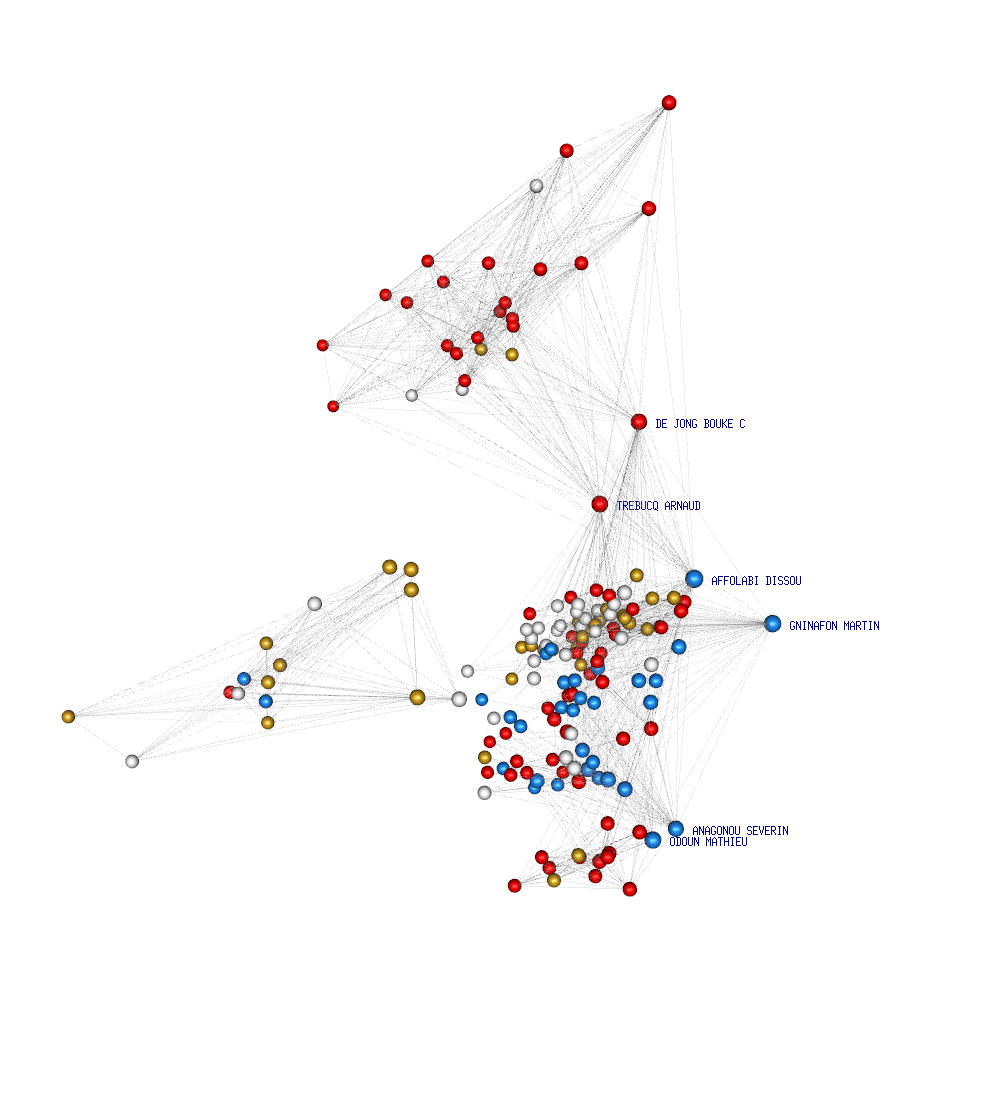
\includegraphics[scale=0.22,trim={5cm 2cm 2cm 0}]{Chapters/tb/statMod/lnm_mod1.png}
\vspace{0px}\\
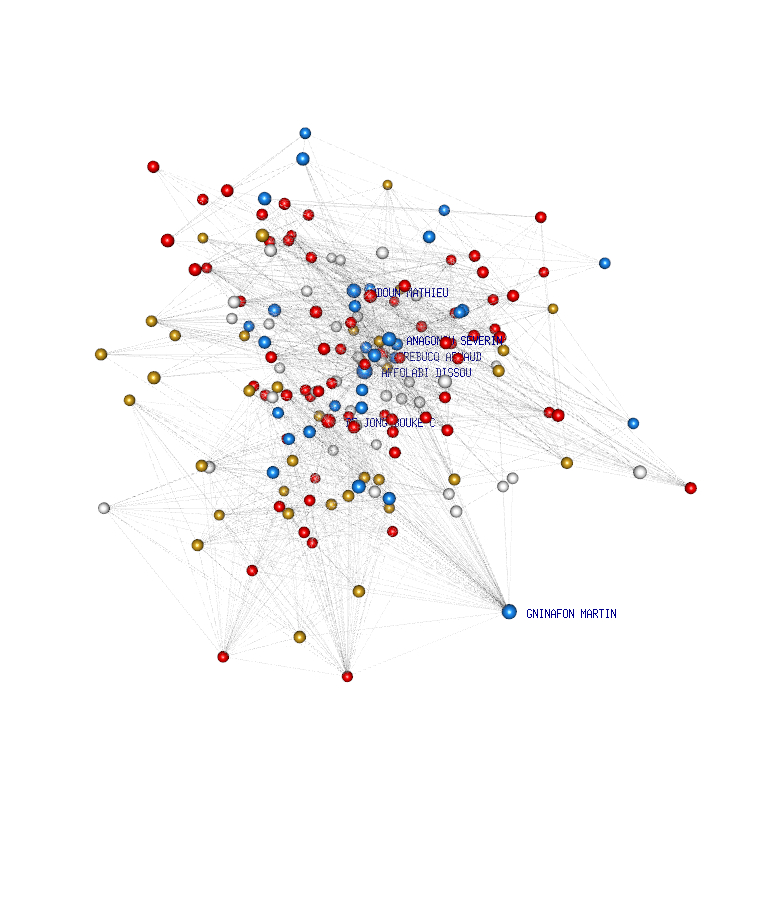
\includegraphics[scale=0.22,trim={5cm 2cm 2cm 5cm}]{Chapters/tb/statMod/lnm_mod5_AllNodal.png}
\vspace{2px}\\
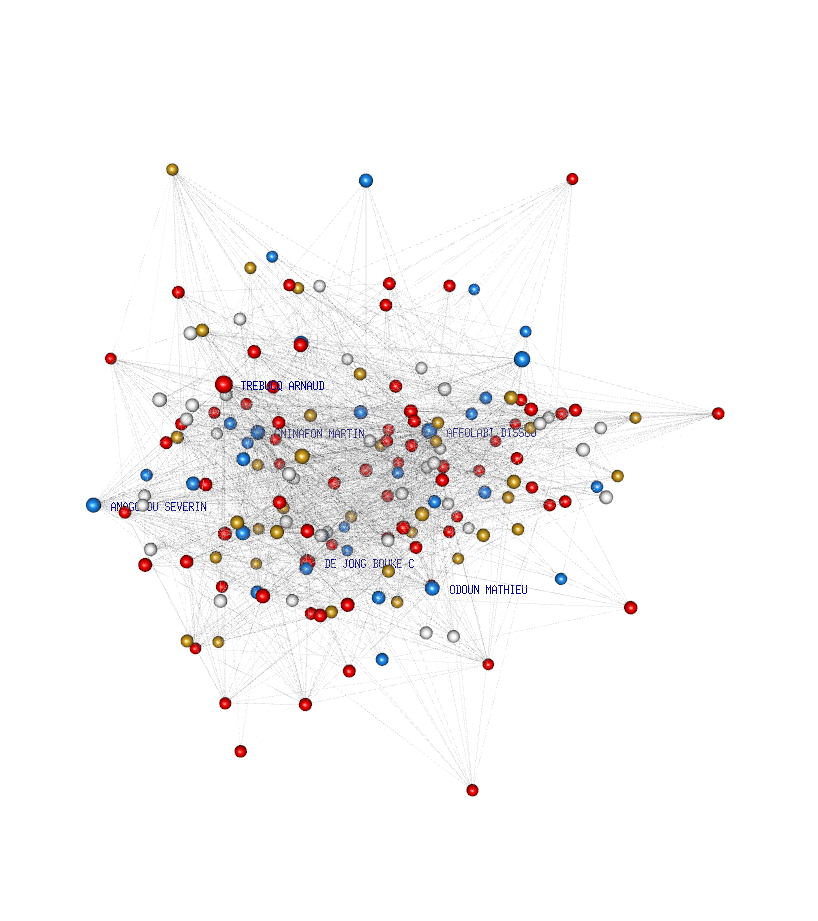
\includegraphics[scale=0.2,trim={5cm 5cm 5cm 5cm}]{Chapters/tb/statMod/lnm_mod7_All.png}
\caption{Visualizations of the TB co-authorship network with layouts determined according to the inferred latent eigenvectors in the LNM models (International (Red); Regional (Gold); Local (Blue); Unknown (White)).
% with no pair-specific covariates (top), nodal covariates (middle), and all covariates (bottom).
}
\label{fig:tb_lnm_viz}
\end{figure}

\begin{figure}[!h]
\centering
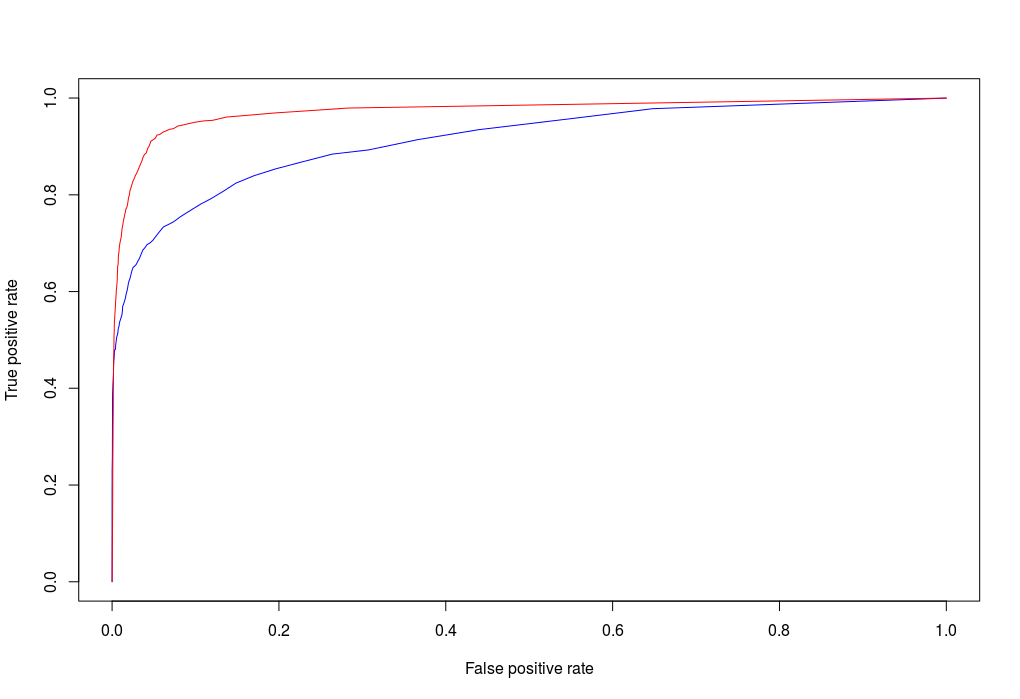
\includegraphics[scale=0.5]{Chapters/tb/statMod/tb_lnm_ROC.png}
\caption{ROC curves comparing the goodness-of fit of the TB co-authorship network for the model specifying (i) no pair specific covariates (blue) and the model specifying (ii) nodal covariates (red)%, and (iii) nodal and dyadic covariates (green), respectively
.}
\label{fig:tb_lnm_roc}
\end{figure}~\\~\\

\pagebreak
\section{Discussion and Conclusion}
\label{sec:tb_discussion}
This chapter provides insights in the structural characteristics of the TB co-authorship network in Benin over the last 20 years. The evolution of the number of publications, authors and collaboration ties suggests a linear growth over the investigation period. We expected such findings given the place of TB in the public health concerns of Benin and the intensive effort towards the reduction of the incidence and the numerous campaigns of sensibilization \cite{world_health_organization_atlas_2016}. The findings from the descriptive analysis suggest that the mechanism underlying the formation of the TB co-authorship network in Benin is not random. However, we found inconclusive evidence of small world properties that further Monte-Carlo simulations disproved. The presence of closed research groups is supected given the non-trivial number of authors with higher order of magnitudes. The observed trend of prolific authors in the TB network to collaborate with less prolific ones is another indication suggesting that TB research is a low productivity research field in Benin. Only 37 published documents were found relevant to the present study. In fact, none of the top 10 key brokers in our TB co-authorship network, was on the list of the top most connected authors and therefore would suggest the relative absence of long publishing tenure authors in the network \cite{li_co-authorship_2013}. \\
The flow of information in the TB co-authorship network in Benin is slow as it only relies on a single author. A study by Salamatia and Soheili \cite{salamati_social_2016} on a co-authorship analysis of Iranian researchers in the field of violence reported similar but less extreme findings. For Bales et al. \cite{bales_social_2008,bales_evolution_2011}, the most important authors in co-authorship networks generally tend to be the ones with the highest degree of collaborations. For information flow, cut vertices provide a better approach to identifying vertices that are important to the long-term substainability of co-authorship networks \cite{kolaczyk_statistical_2014}. The only author identified as a cut vertex is therefore the most important author for information flow.\\
Our observed network has unexpected properties compared to classic small-world networks. Our TB co-authorship network displays properties that are more extreme than those of small-world and preferential attachement networks contradicting previous studies reporting co-authorship network as having small-world or preferential attachment properties \cite{gonzalez-alcaide_scientific_2012,wagner_network_2005}.\\
As the first advanced statistical model we applied to this network, the SBM identified heterogeneous classes with higher probabilities towards inter class ties establishment. This observation is different from what we observed for the malaria and the HIV/AIDS co-authorship network which both display low inter class probabilities and higher intra class probabilities of tie formation. \\
As in the malaria and the co-authorship network, the ERGM and TERGM results suggest that authors within the TB co-authorship network are more likely to establish collaboration ties within their research groups or communities. Although marginal, factors such as number of publications, number of citations and number of collaborations are associated to higher likelihood to establishing collaboration ties, confirming therefore our first hypothesis. Adding temporal dependencies to our ERGM models tremendously improved the fitness of the model to the observed network data, but at a cost of decreased performance compared to the model without temporal dependencies.\\
We expected the ERGMs and TERGMs containing ERGM structural terms to converge for the TB co-authorship network given its relatively smaller size. Unfortunately, as for the malaria and the HIV/AIDS co-authorship networks, adding such terms to the models proved computationally expensive. None of the models converged after $1,000$ iterations. We therefore, suspect the complexity of the network to have prevented the convergence of the models containing structural ERGM terms \cite{schmid_exponential_2017}. \\ 
With the LNM, we complement the ERGM and TERGM by adding an extra layer of analysis. Visualizing the effect of geography on the structure of the network, we notice that none of the nodal or dyadic covariates played a significant role in the spatial distribution of the network. Such an observation contradicts that of the HIV/AIDS co-authorship network. The cluster demarcation observed with the null LNM suggests that distance does play a significant role in collaboration tie formation in the TB co-authorship network. \\
As the co-infection TB-HIV/AIDS continues to be an important aspect of the public health strategies in the Republic of Benin, consolidating the knowledge generated from the TB-related research is crucial. Furthermore, public health policies must empower and reinforce the different research groups or communities involved in the research effort. Our results suggest a need for a continuous support to the TB research network, considering its low productivity status in Benin. Such actions will help stabilize the research groups already involved in TB research and promote the junior scientists in the field. We finally believe that such measures will ultimately insure the long-term sustainability of the TB co-authorship and collaborative research network in Benin.

